\documentclass{article}
\usepackage[preprint,nonatbib]{neurips_2025}
\usepackage{fontspec}
\setmainfont{Liberation Serif}
\setsansfont{Liberation Sans}
\usepackage{graphicx}
\usepackage{booktabs}
\usepackage{array}
\usepackage{tabularx}
\usepackage{makecell}
\usepackage{float}
\usepackage{placeins}
\usepackage{enumitem}
\usepackage{hyperref}
\usepackage{xcolor}
\usepackage{caption}
\captionsetup{font=small,labelfont=bf}
\setlist[itemize]{leftmargin=*,nosep}
\setlist[enumerate]{leftmargin=*,nosep}
\graphicspath{{./}}

\title{Part 2 EDA/Data Storytelling: Từ doanh thu đến quyết định vận hành cho e-commerce fashion Việt Nam}
\author{Datathon 2026 -- The Gridbreakers\\Part 2 EDA Report}

\begin{document}
\maketitle

\begin{abstract}
Báo cáo này chỉ dùng 13 bảng dữ liệu thật dành cho EDA: products, customers, promotions, geography, orders, order\_items, payments, shipments, returns, reviews, sales, inventory và web\_traffic. Hai file phục vụ Part 3/submission không được đọc hoặc dùng làm bằng chứng. Câu chuyện chính là doanh nghiệp không thiếu tín hiệu, mà đang có ba điểm nghẽn có thể hành động: nhu cầu gãy mạnh từ 2019 và mùa cao điểm nằm ở Q2; lợi nhuận tập trung vào Streetwear/SKU chọn lọc trong khi promotion có dấu hiệu phòng thủ; và tồn kho vừa stockout vừa overstock, làm mất cơ hội ở SKU nóng và khóa vốn ở SKU lạnh.
\end{abstract}

\section{Cách đọc báo cáo}
Report này đi theo dòng chảy của một đơn hàng e-commerce: nhu cầu thị trường tạo traffic và đơn hàng, đơn hàng rơi vào danh mục/SKU cụ thể, promotion thay đổi giá trị đơn, trải nghiệm giao nhận và return quyết định phần doanh thu giữ lại, còn inventory quyết định doanh nghiệp có đủ hàng để bán đúng mùa hay không. Rubric Part 2 vẫn được giữ trong cấu trúc lập luận: mỗi phát hiện đều bắt đầu từ số liệu mô tả, đi tiếp sang chẩn đoán, rồi kết thúc bằng hệ quả kinh doanh và hướng hành động. Phần modeling Part 3 chỉ được nhắc ngắn ở cuối.

\textbf{Data guardrail.} Script sinh report là \texttt{report/build\_part2\_report.py}. Danh sách đọc dữ liệu được hard-code đúng 13 bảng EDA; \texttt{sales\_test.csv} và \texttt{sample\_submission.csv} nằm trong danh sách cấm. Tổng phạm vi train là 2012-07-04--2022-12-31 với 3,833 ngày doanh thu, tổng doanh thu 16.43 tỷ VND, gross margin 13.8\%.

\begin{table}[H]
\caption{Audit 13 bảng dùng trong EDA. Missing cao ở promo fields là nullable theo schema, không phải lỗi dữ liệu.}
\centering
\scriptsize
\begin{tabularx}{\linewidth}{lrrlX}
\toprule
Table & Rows & Cols & Date range & Max missing column \\
\midrule
products & 2,412 & 8 & -- & product\_id (0.00\%) \\
customers & 121,930 & 7 & 2012-01-17--2022-12-31 & customer\_id (0.00\%) \\
promotions & 50 & 10 & 2013-01-31--2022-12-31 & applicable\_category (80.00\%) \\
geography & 39,948 & 4 & -- & zip (0.00\%) \\
orders & 646,945 & 8 & 2012-07-04--2022-12-31 & order\_id (0.00\%) \\
order\_items & 714,669 & 7 & -- & promo\_id\_2 (99.97\%) \\
payments & 646,945 & 4 & -- & order\_id (0.00\%) \\
shipments & 566,067 & 4 & 2012-07-04--2022-12-31 & order\_id (0.00\%) \\
returns & 39,939 & 7 & 2012-07-11--2022-12-31 & return\_id (0.00\%) \\
reviews & 113,551 & 7 & 2012-07-10--2022-12-31 & review\_id (0.00\%) \\
sales & 3,833 & 3 & 2012-07-04--2022-12-31 & Date (0.00\%) \\
inventory & 60,247 & 17 & 2012-07-31--2022-12-31 & snapshot\_date (0.00\%) \\
web\_traffic & 3,652 & 7 & 2013-01-01--2022-12-31 & date (0.00\%) \\
\bottomrule
\end{tabularx}
\end{table}

\section{Câu chuyện chính}
Nhìn từ xa, doanh nghiệp giống như đang gặp một bài toán forecasting: cần dự báo doanh thu ngày. Nhưng khi nối 13 bảng lại với nhau, vấn đề hiện ra rộng hơn. Đây là một retailer fashion e-commerce có demand đã đổi trạng thái từ 2019, mùa cao điểm nằm ở Q2 thay vì cuối năm, và phần lớn revenue phụ thuộc vào Streetwear. Ở tầng vận hành, promotion đang được dùng nhiều vào những ngày yếu, return chủ yếu đến từ vấn đề size/expectation, còn inventory vừa stockout vừa overstock. Nói cách khác, doanh nghiệp không thiếu dữ liệu; vấn đề là các quyết định về mùa vụ, SKU, promotion và tồn kho đang chưa cùng nhịp.

\section{Cú gãy 2019: doanh thu rơi vì mất lượng đơn}
Điểm ngoặt lớn nhất của chuỗi doanh thu không nằm ở năm 2020 mà đã xuất hiện trong 2019. Revenue năm 2019 giảm -38.6\% YoY; sau điểm gãy này, daily revenue trung bình giai đoạn 2019--2022 thấp hơn 40.5\% so với 2012--2018. Đến 2022 doanh thu có phục hồi 12.1\%, nhưng vẫn chưa trở lại nền trước 2019.

Điều quan trọng là cú rơi này không đến từ việc khách mua đơn nhỏ hơn. Decomposition cho thấy số đơn 2019 giảm -40.2\%, units giảm -40.0\%, trong khi AOV lại tăng 2.7\%. Vì vậy tín hiệu gần nhất trong dữ liệu là demand/order flow bị mất, không phải basket value suy yếu. Nếu doanh nghiệp lập kế hoạch tồn kho và ngân sách bằng cách trung bình hóa toàn bộ lịch sử 2012--2022, các năm trước 2019 sẽ kéo kế hoạch lên quá cao. Baseline vận hành nên bắt đầu từ giai đoạn hậu 2019, rồi dùng order count và units sold làm early-warning thay vì chờ revenue tổng phản ứng.

\begin{figure}[H]
\centering
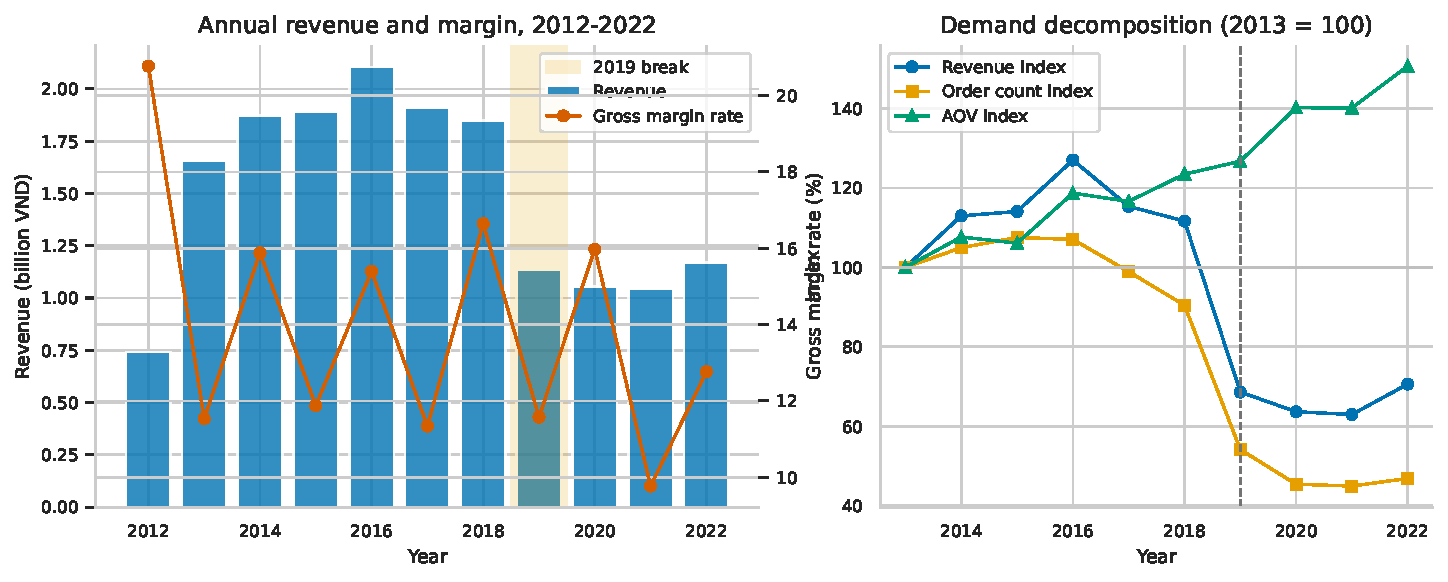
\includegraphics[width=\linewidth]{figures/01_revenue_decomposition.pdf}
\caption{Revenue break và decomposition. Sources: \texttt{sales}, \texttt{orders}, \texttt{order\_items}, \texttt{products}.}
\end{figure}

\section{Mùa bán hàng thật sự bắt đầu trước mùa hè}
Sau cú gãy demand, câu hỏi tiếp theo là doanh nghiệp nên chuẩn bị cho mùa nào. Dữ liệu trả lời khá rõ: tháng 5 có daily revenue cao hơn trung bình 53.4\%, còn tháng 12 thấp hơn 41.1\%. Đây là một pattern quan trọng vì nó đi ngược trực giác phổ biến rằng fashion sẽ cao điểm cuối năm.

Khi tách theo category, seasonality cũng không còn là một đường duy nhất. Streetwear peak tháng 5, GenZ peak tháng 6, trong khi Outdoor peak tháng 12. Mix category kéo tổng doanh nghiệp về Q2, nhưng Outdoor vẫn cần cách nhìn riêng. Vì vậy lịch mua hàng, lịch campaign và lịch replenishment nên bắt đầu từ tháng 3 cho Streetwear/Casual/GenZ, đồng thời giữ ngân sách và hàng Outdoor cho tháng 12 và các vùng phù hợp.

\begin{figure}[H]
\centering
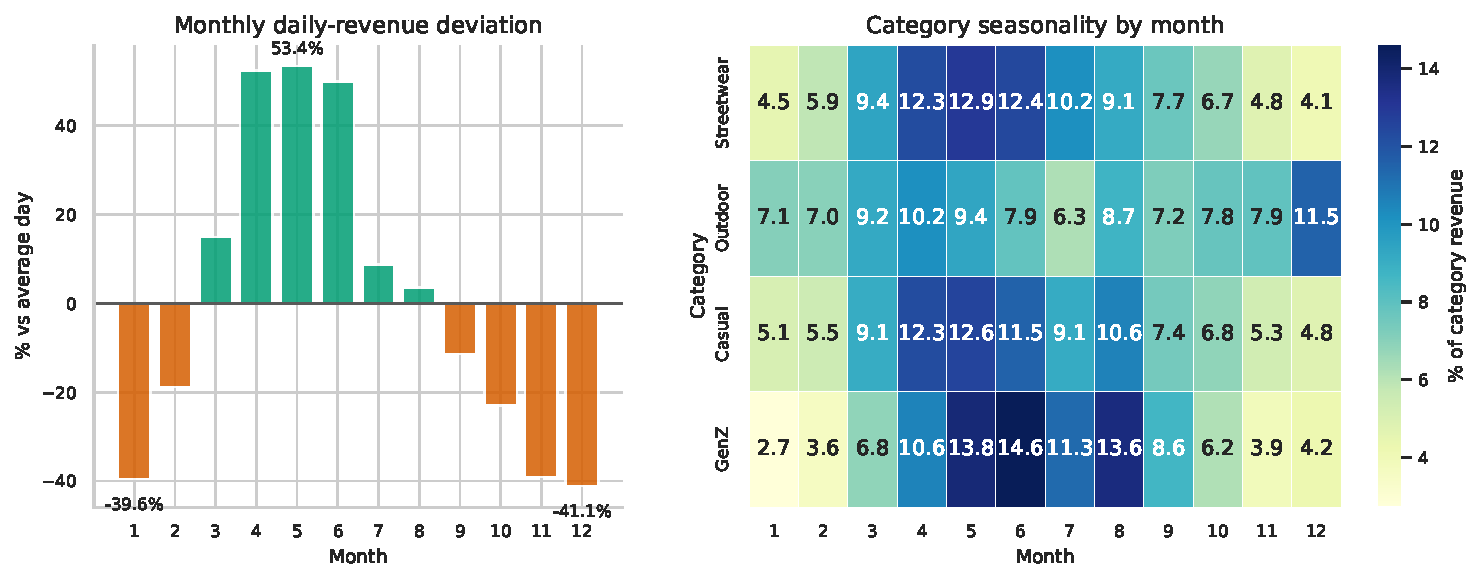
\includegraphics[width=\linewidth]{figures/02_seasonality_category.pdf}
\caption{Seasonality tổng và theo category. Sources: \texttt{sales}, \texttt{orders}, \texttt{order\_items}, \texttt{products}.}
\end{figure}

\section{Revenue đến từ Streetwear, nhưng lợi nhuận nằm ở SKU được chọn đúng}
Nếu chỉ nhìn revenue tổng, doanh nghiệp gần như là một doanh nghiệp Streetwear: category này chiếm 79.9\% revenue và HHI category đạt 0.663. Mức tập trung này vừa là lợi thế nhận diện, vừa là rủi ro: bất kỳ shock nào ở Streetwear cũng sẽ đi thẳng vào P\&L tổng.

Nhưng trong Streetwear, không phải SKU nào cũng đáng scale như nhau. SKU gross-margin cao nhất là SaigonFlex UM-43, tạo 130.5 triệu VND gross margin. Biểu đồ profit pool cho thấy bestseller theo units không tự động là profit driver vì margin rate, price point và promo dependence khác nhau. Quyết định merchandising nên chuyển từ ``bán nhiều thì nhập nhiều'' sang gross-margin by SKU/month: bảo vệ SKU profit driver trước mùa cao, còn các SKU volume lớn nhưng margin mỏng phải có guardrail rõ ràng.

\begin{figure}[H]
\centering
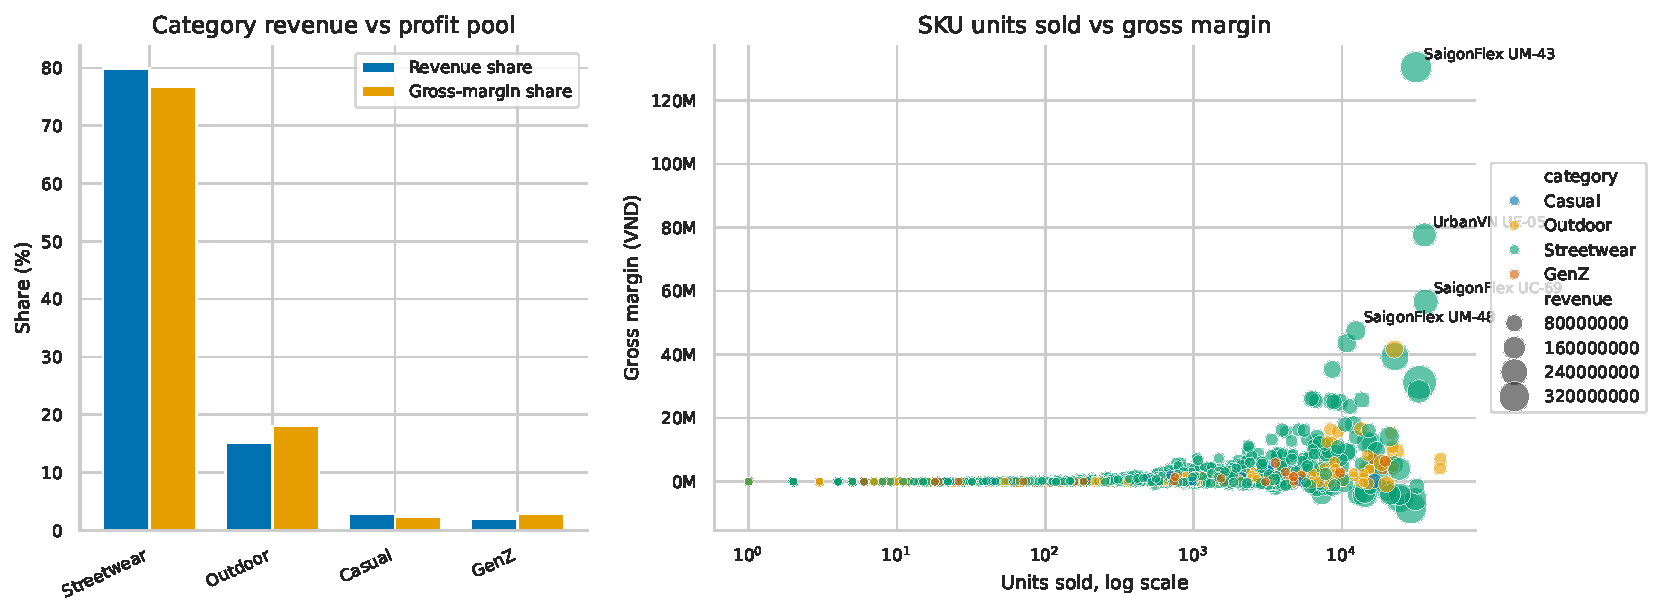
\includegraphics[width=\linewidth]{figures/03_profit_pool.pdf}
\caption{Profit pool theo category và SKU. Sources: \texttt{products}, \texttt{order\_items}.}
\end{figure}

\section{Promotion đang giống phanh giảm rủi ro hơn là bàn đạp tăng trưởng}
Promotion là nơi dễ bị diễn giải quá nhanh. Trong dữ liệu này, ngày có trên 50\% đơn dùng promo lại có median revenue thấp hơn 13.3\% so với ngày có dưới 10\% đơn dùng promo; Spearman giữa promo share và revenue là -0.114. Con số này không chứng minh promo làm giảm revenue, nhưng nó phá vỡ giả định ``cứ tăng khuyến mãi là tăng doanh thu''.

Cách đọc hợp lý hơn là promotion đang được dùng phòng thủ: team có thể tung coupon vào ngày dự kiến yếu, hoặc discount đang rơi vào khách vốn đã định mua. Nếu không đo uplift thật, doanh nghiệp có thể đổi gross margin lấy một lượng revenue không tăng tương ứng. Promotion nên được quản trị như một intervention có holdout/A-B test, tách rõ campaign tăng trưởng và campaign cứu ngày yếu, đồng thời đặt margin guardrail ở cấp SKU.

\begin{figure}[H]
\centering
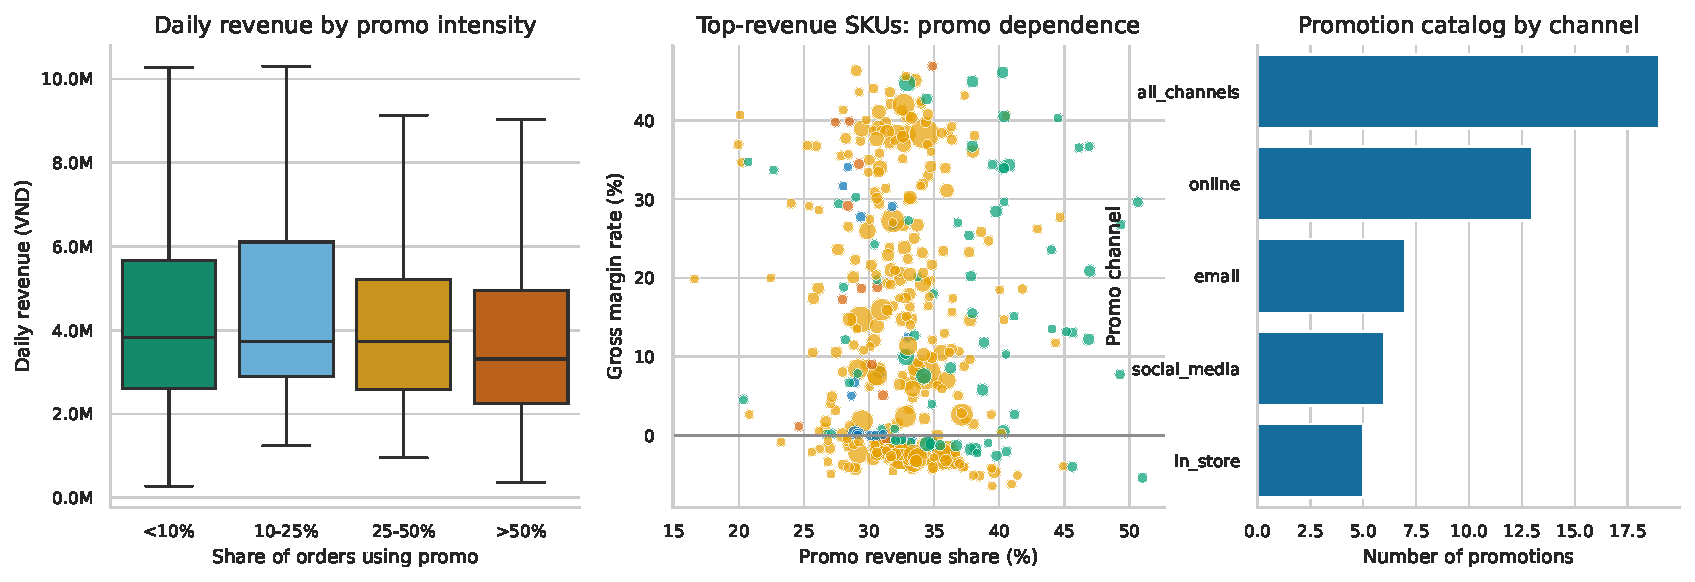
\includegraphics[width=\linewidth]{figures/04_promotion_guardrails.pdf}
\caption{Promo intensity, promo dependence và catalog khuyến mãi. Sources: \texttt{orders}, \texttt{order\_items}, \texttt{promotions}, \texttt{products}.}
\end{figure}

\section{Xương sống thương mại là khách quay lại và search intent}
Sau category và promo, lớp tiếp theo là khách hàng. Top 20\% khách tạo 60.6\% revenue; 75.2\% khách đã mua hơn một đơn. Đây là một doanh nghiệp có core cohort mạnh, không chỉ sống bằng acquisition mới.

Kênh cũng củng cố nhận định đó. Organic search đóng 28.0\% revenue, còn credit card chiếm 55.0\% payment value. Người mua có vẻ đến với ý định khá rõ, rồi quay lại nhiều lần. Điều này khiến retention quan trọng hơn vẻ ngoài của traffic volume: mất nhóm khách core sẽ đắt hơn nhiều so với một biến động nhỏ ở acquisition. Doanh nghiệp nên theo dõi active repeat customers 30 ngày như một KPI demand, tạo early-access/VIP drop trước mùa cao, và đảm bảo checkout/payment flow ổn định cho nhóm thanh toán bằng thẻ.

\begin{figure}[H]
\centering
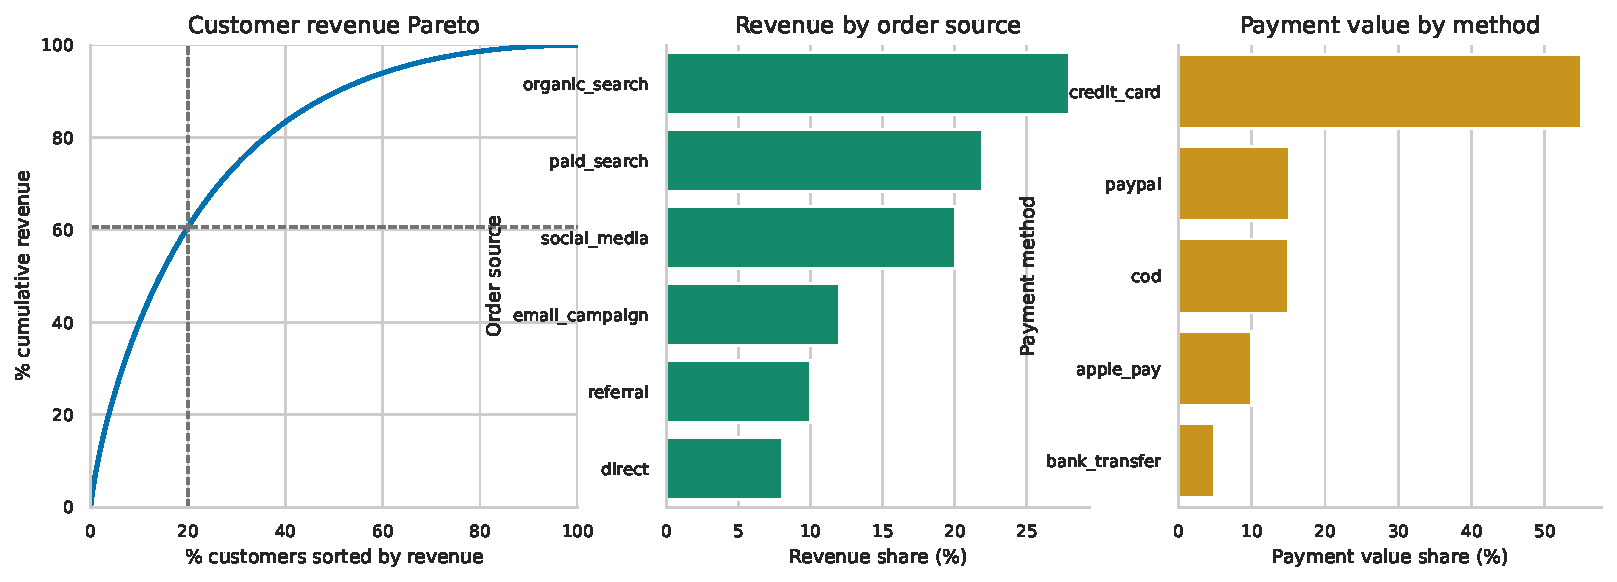
\includegraphics[width=\linewidth]{figures/05_customer_channel_payment.pdf}
\caption{Customer Pareto, order source và payment mix. Sources: \texttt{customers}, \texttt{orders}, \texttt{order\_items}, \texttt{payments}.}
\end{figure}

\section{Return leakage không nằm ở một category xấu}
Doanh thu không kết thúc ở checkout; một phần bị rò qua return. Lý do lớn nhất là \texttt{wrong\_size}, chiếm 34.7\% returned units và 34.6\% refund. Nếu return tập trung vào một category, giải pháp có thể là sửa line sản phẩm đó. Nhưng ở đây return rate giữa category chỉ dao động từ 3.3\% đến 3.5\%, còn correlation giữa delivery days và rating gần như bằng 0 (-0.006).

Vì vậy vấn đề có vẻ nằm ở cơ chế mua hàng: size guide, fit expectation, mô tả sản phẩm, hoặc chính sách đổi trả chung. Hành động tốt nhất không phải cắt một category, mà là giảm sai lệch trước checkout: chuẩn hóa size chart, hiển thị fit notes theo SKU, cảnh báo những biến thể hay bị trả và audit mô tả sản phẩm cho nhóm \texttt{not\_as\_described}.

\begin{figure}[H]
\centering
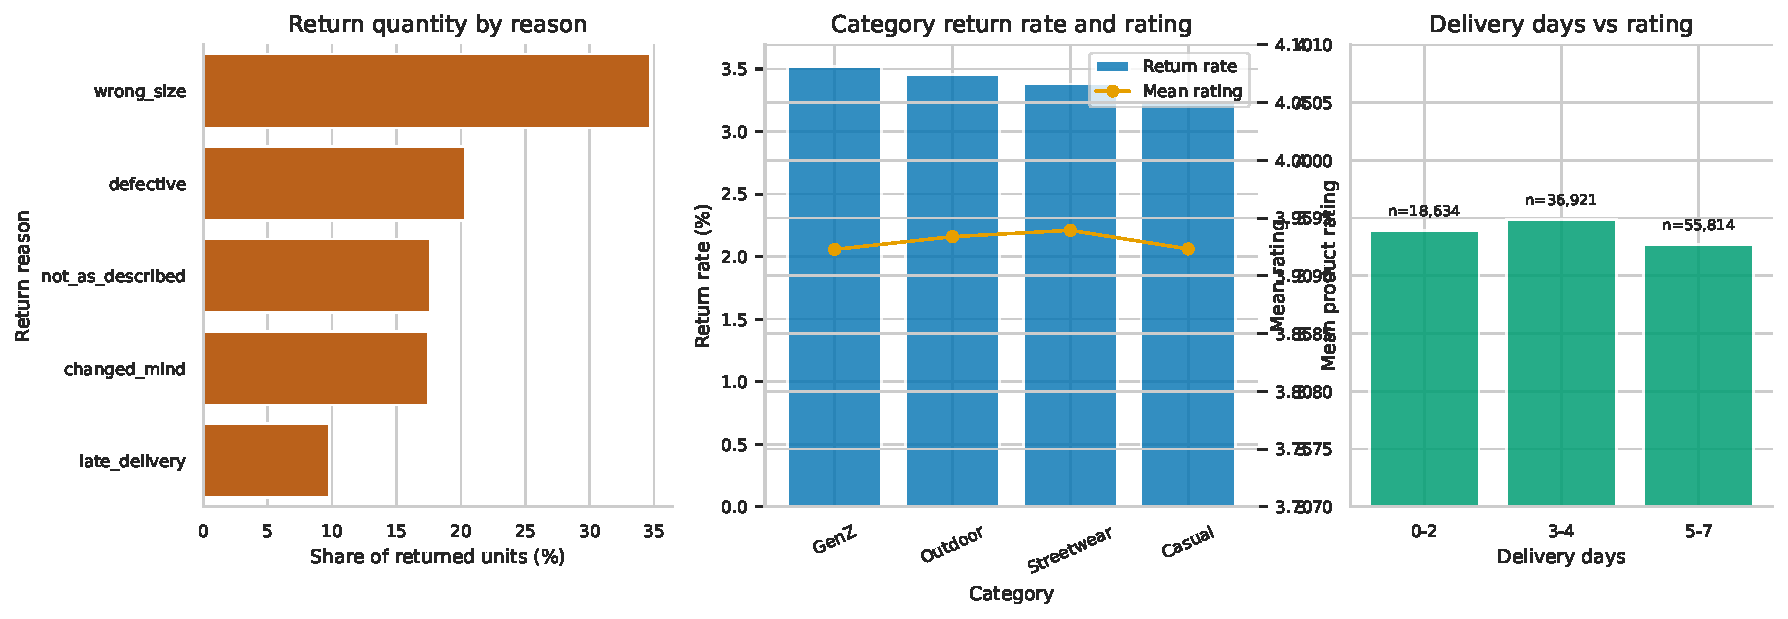
\includegraphics[width=\linewidth]{figures/06_returns_experience.pdf}
\caption{Return reasons, category return-rate/rating và delivery-rating check. Sources: \texttt{returns}, \texttt{reviews}, \texttt{shipments}, \texttt{products}, \texttt{order\_items}.}
\end{figure}

\section{Địa lý không chỉ là nơi bán nhiều hay ít}
Khi đặt demand lên bản đồ, East là vùng lớn nhất với 46.5\% revenue, Central đóng 30.1\%, và West đóng 23.4\%. Nhưng điểm đáng chú ý hơn là mix category: Outdoor chiếm 26.2\% revenue ở West, cao hơn nhiều so với 11.8\% ở East.

Điều này biến geography từ một bảng tham chiếu thành input cho merchandising. Một plan toàn quốc có thể đúng về tổng revenue nhưng sai về category allocation. Streetwear nên được scale mạnh hơn ở East/Central; Outdoor cần được nhìn riêng ở West và gắn với mùa peak của category này.

\begin{figure}[H]
\centering
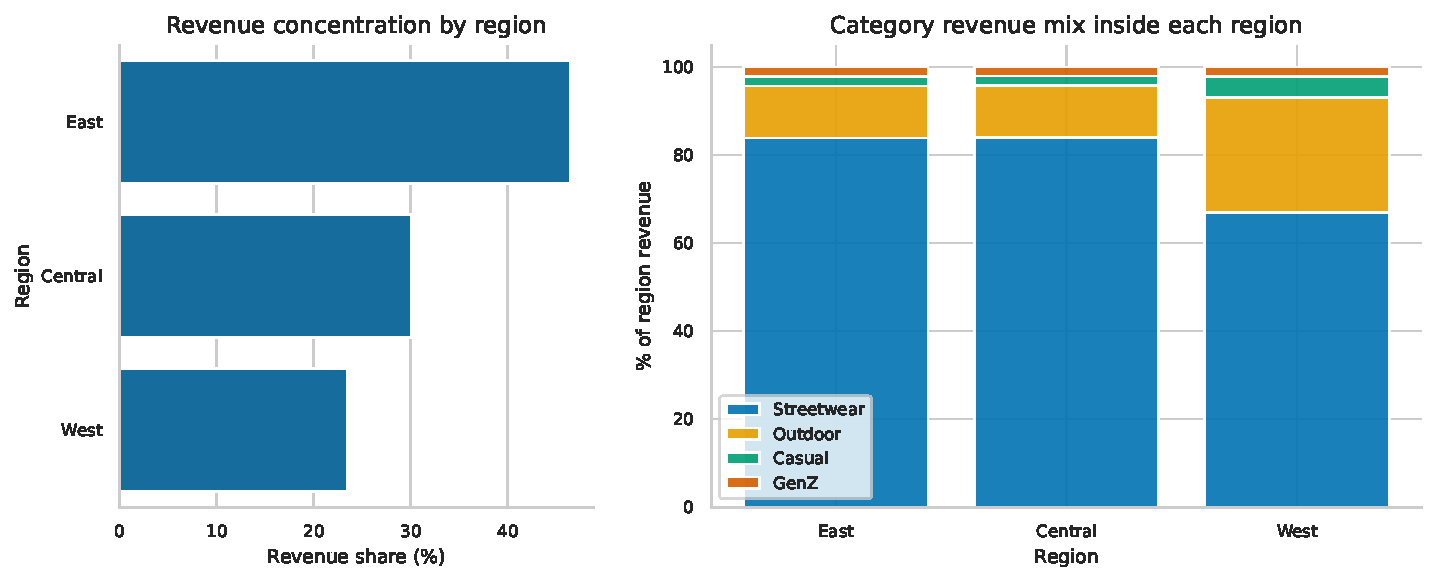
\includegraphics[width=\linewidth]{figures/07_geography_mix.pdf}
\caption{Revenue concentration và category mix theo vùng. Sources: \texttt{geography}, \texttt{orders}, \texttt{order\_items}, \texttt{products}.}
\end{figure}

\section{Nút thắt vận hành: thiếu hàng nóng, thừa hàng lạnh}
Inventory là nơi câu chuyện quay lại quyết định thực thi. Trong năm 2022, average monthly stockout rate đạt 66.6\%, overstock rate cũng lên tới 76.7\%, trong khi sell-through trung bình chỉ 13.6\%. Hai chỉ số stockout và overstock cùng cao cho thấy doanh nghiệp không chỉ thiếu hàng; doanh nghiệp đang phân bổ sai SKU/tháng.

Hệ quả rất thực tế: SKU nóng làm mất revenue vì stockout, còn SKU lạnh khóa vốn vì days-of-supply dài. Trước mùa cao Q2, ưu tiên không phải tăng nhập toàn danh mục mà là reallocation: replenish high-demand stockout SKU, đồng thời markdown hoặc liquidate chronic overstock với guardrail margin.

\begin{figure}[H]
\centering
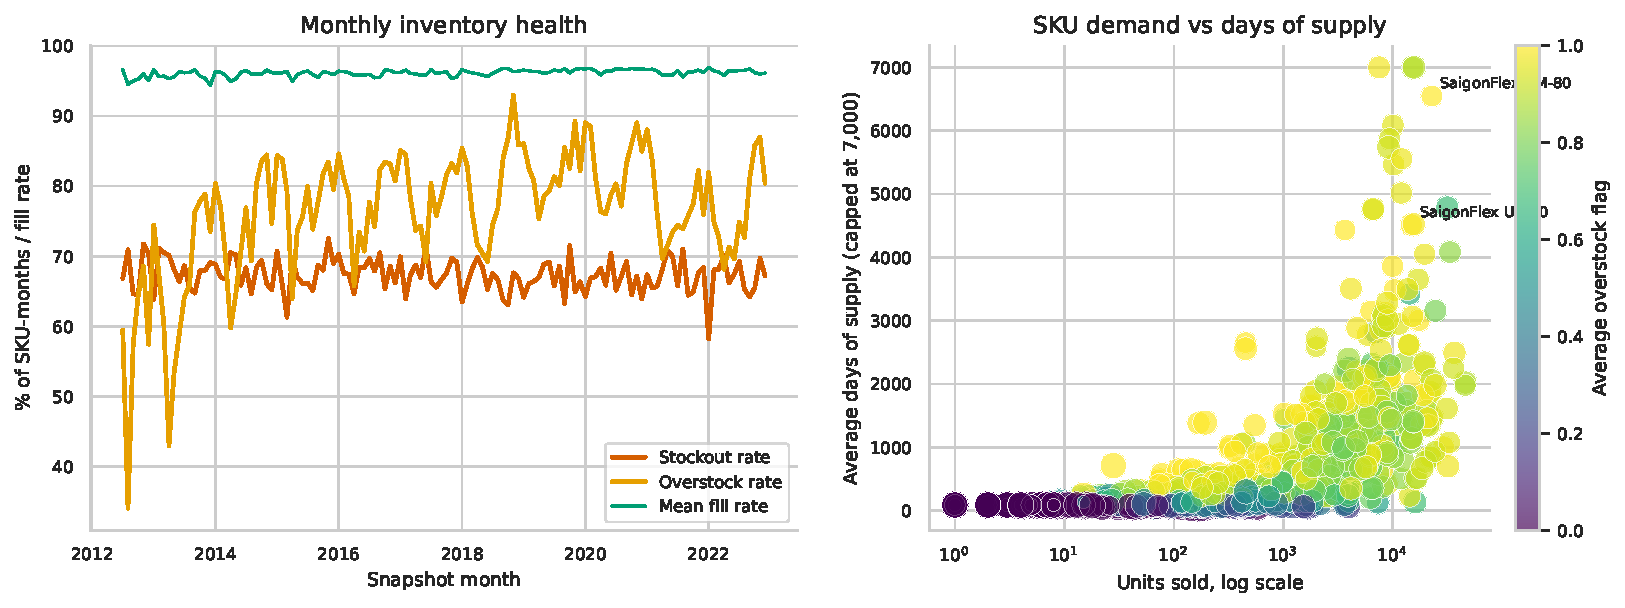
\includegraphics[width=\linewidth]{figures/08_inventory_misalignment.pdf}
\caption{Inventory health theo tháng và SKU-level demand vs days-of-supply. Sources: \texttt{inventory}, \texttt{products}, \texttt{order\_items}.}
\end{figure}

\section{Traffic là tín hiệu phụ, không phải câu trả lời}
Web traffic vẫn có giá trị, nhưng không đủ mạnh để một mình giải thích revenue. Spearman giữa sessions và revenue là 0.368; unique visitors là 0.369. Kiểm tra lead/lag cũng không làm tín hiệu mạnh lên nhiều: điểm tốt nhất của sessions chỉ đạt 0.373 tại lag 1 ngày.

Điều này hợp lý sau khi đã nhìn các tầng trước. Revenue bị chi phối bởi mùa vụ, category mix, promotion, repeat customers và inventory gate. Đẩy traffic vào một SKU đang stockout hoặc vào một tháng trái mùa sẽ không tạo revenue tương ứng. Traffic nên được dùng như feature phụ và nên đo theo source/conversion/value, đặc biệt khi quyết định paid media phải đi cùng trạng thái tồn kho.

\begin{figure}[H]
\centering
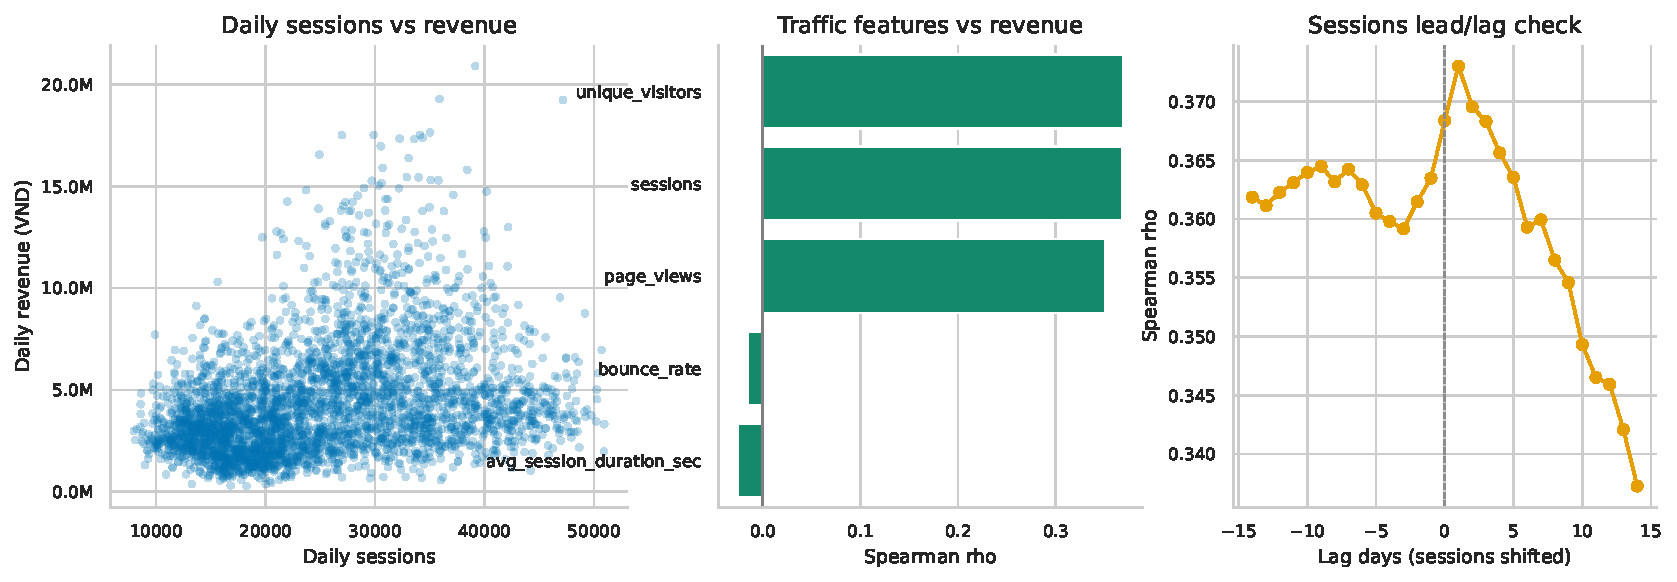
\includegraphics[width=\linewidth]{figures/09_web_traffic_signal.pdf}
\caption{Traffic signal strength và lead/lag check. Sources: \texttt{web\_traffic}, \texttt{sales}.}
\end{figure}

\section{Bản đồ hành động}
Sau khi nối các phần lại, các quyết định ưu tiên có thể tóm lại như sau. Bảng này không thay thế câu chuyện phía trên; nó là bản đồ triển khai để team commercial, marketing và operations cùng nhìn một nguồn sự thật.
\begin{table}[H]
\caption{Prescriptive summary: quyết định kinh doanh gắn với bằng chứng.}
\centering
\scriptsize
\begin{tabularx}{\linewidth}{r l X X}
\toprule
\# & Nhóm quyết định & Bằng chứng chính & Việc nên làm \\
\midrule
1 & Kế hoạch nhu cầu & Revenue 2019 giảm 38.6\% YoY, số đơn giảm 40.1\%; daily mean hậu 2019 thấp hơn 40.5\% so với 2012-2018. & Lấy hậu 2019 làm baseline vận hành; không cho các năm đầu kéo kế hoạch tồn kho/ngân sách lên quá cao. \\
2 & Merchandising theo mùa & Tháng 5 cao hơn average day 53.4\%; tháng 12 thấp hơn 41.1\%; peak month khác nhau theo category. & Chuẩn bị mua hàng/content/stock từ tháng 3-6; giữ Outdoor allocation riêng cho tháng 12 và vùng West. \\
3 & Quản trị promotion & Ngày có >50\% đơn dùng promo có median revenue thấp hơn 13.3\% so với ngày <10\% promo. & Dùng promo như intervention có đo uplift và margin guardrail, không chạy blanket như đòn bẩy mặc định. \\
4 & Retention và kênh bán & Top 20\% khách tạo 60.6\% revenue; 75.2\% khách có đơn là repeat buyers. & Bảo vệ cohort giá trị cao bằng early access/personalized drops trước mùa peak. \\
5 & Rò rỉ qua return & wrong\_size chiếm 34.7\% return quantity và 34.6\% refund; return rate giữa category rất sát nhau. & Sửa size guidance và expectation trên product page ở cấp hệ thống trước khi nhắm vào một category. \\
6 & Phân bổ tồn kho & Năm 2022 có stockout rate 66.6\% và overstock rate 76.7\% cùng lúc. & Reallocate ở cấp SKU: replenish SKU nhu cầu cao bị stockout và xử lý chronic overstock. \\
7 & Traffic và tín hiệu dự báo & Sessions chỉ tương quan 0.368 với revenue; lead/lag tốt nhất là 0.373 tại lag +1. & Dùng traffic như tín hiệu phụ; đo conversion/value theo source thay vì tối ưu volume thuần. \\
\bottomrule
\end{tabularx}
\end{table}

\section{Part 3 note và giới hạn suy luận}
Part 3/modeling không phải trọng tâm của report này. Nếu template yêu cầu nhắc, EDA gợi ý các feature hợp lệ từ train-only data: post-2019 regime indicator, month/day-of-week/Fourier seasonality, promo share lag, active repeat customers, category mix, web traffic, inventory stockout/overstock lag và return/refund lag. Không có số liệu test/submission nào được dùng trong EDA.

Các claim causal được giữ thận trọng. Đặc biệt, promo--revenue là quan hệ quan sát nên chỉ hỗ trợ giả thuyết về defensive promotion/cannibalization; muốn đo uplift cần experiment hoặc thiết kế quasi-experiment. Inventory không có warehouse/region dimension nên region allocation là khuyến nghị merchandising, không phải tối ưu kho vùng đầy đủ.

\end{document}
